



\section{Methodology}
In this section, we first introduce Infinity-Doc-400K, our large-scale multimodal dataset for end-to-end scanned document parsing. We then describe our rule-based multi-aspect reward framework, which integrates edit distance, paragraph count, and order criteria under a unified reinforcement learning objective optimized via Group Relative Policy Optimization (GRPO). 

% Finally, we detail a curriculum learning strategy that schedules training samples by structural difficulty to stabilize and accelerate convergence on complex documents.






\subsection{Infinity-Doc-400K and Generation Pipelines }


We introduce Infinity-Doc-400K, a large-scale, multimodal dataset of 400,066 richly annotated documents for end-to-end scanned document parsing. Unlike prior benchmarks that target isolated subtasks (e.g., layout detection, OCR, or table recognition), Infinity-Doc-400K provides holistic supervision by pairing rendered scanned document pages with their ground-truth Markdown representations. This design enables training and evaluating models that directly translate visual inputs to layout outputs without relying on brittle, multi-stage pipelines. As shown in Table \ref{tab:all-1}, compared to existing works, Infinity-Doc-400K not only significantly enhances task diversity but also substantially improves overall data quality through our proposed synthetic generation mechanism. More details on the data distribution and quality control are provided in the Data Details section of the Appendix.


 

To construct Infinity-Doc-400K, we design a dual-pipeline framework that integrates both synthetic and real-world document generation, as illustrated in Figure~\ref{fig:example111}. This design addresses a critical limitation of traditional data construction pipelines, which often rely on weak supervision and pseudo-labeling from a single model applied to crawled, scanned documents. These pipelines frequently suffer from noisy, misaligned, or incomplete annotations, especially in complex layouts or multilingual content, thus hindering model performance and generalization. To overcome these issues, our dual-pipeline framework is motivated by the need to balance annotation quality and structural diversity. The synthetic branch provides highly accurate, clean, and precisely aligned annotations at scale, while the real-world branch introduces naturally occurring layout variability and semantic richness, which are essential for building models that generalize robustly in practical applications. 


\paragraph{Real-World Data} We develop a real-world data construction pipeline to capture the structural complexity and natural layout variability of documents across practical domains. We collect diverse scanned documents from sources such as financial reports, medical records, academic papers, books, magazines, and web pages, covering both dense and sparse content layouts. To generate structural annotations, we adopt a multi-expert strategy, where specialized models handle different structural elements, such as layout blocks, texts, formulas, and tables. For example, overall layouts are analyzed by a visual layout model~\citep{huang2022layoutlmv3pretrainingdocumentai}, formula regions are processed by a dedicated formula recognition model~\citep{wang2024unimernetuniversalnetworkrealworld}, and tables are parsed by a transformer-based table extractor~\citep{Nougat}. A cross-validation mechanism is then applied to filter out inconsistencies by comparing the outputs of expert models and VLMs. Only regions with consistent predictions across models are retained as high-confidence pseudo-ground-truth annotations. This layout-aware filtering results in a rich and reliable dataset that reflects the complexity of real-world documents and supports robust document parsing model training.







\paragraph{Synthetic Data} We design a synthetic data construction pipeline. We collect text and images from sources such as Wikipedia, web crawlers, and online corpora, and use Jinja~\citep{nipkow2003jinja} templates to inject sampled content into predefined single-, double-, or triple-column HTML layouts. These pages are rendered into scanned documents using a browser engine, followed by automated filtering to remove low-quality or overlapping images. Ground-truth annotations are extracted by parsing the original HTML to produce aligned Markdown representations.  This synthetic approach not only significantly reduces construction costs and ensures annotation accuracy and structural diversity, but more importantly, it addresses the longstanding issue of imprecise or inconsistent supervision commonly found in pseudo-labeled datasets, providing high-quality and well-aligned supervision for training end-to-end models.



\paragraph{Quality Control Measures} To ensure reliable annotations at scale, we designed a hybrid quality control strategy for Infinity-Doc-400K. First, three domain experts with doctoral degrees in document analysis manually inspected about 5\% of the data. Their feedback not only identified potential errors but also served as a quality anchor for evaluating annotation consistency. Guided by these inspections, we iteratively refined the screening rules no fewer than five times, continuously improving the labeling pipeline. Finally, to achieve scalability, we employed a model-based cross-verification mechanism: multiple models generated annotations for real-world samples, with high-consistency outputs retained and inconsistent cases fed back into further rule refinement. This layered framework—anchored by expert inspection, strengthened through iterative rule optimization, and scaled via model cross-checking—effectively balances annotation reliability with dataset scalability.




\begin{figure}[t]
  \centering
  % 插入图片，options 中可以设置宽度、高度、缩放比例等
  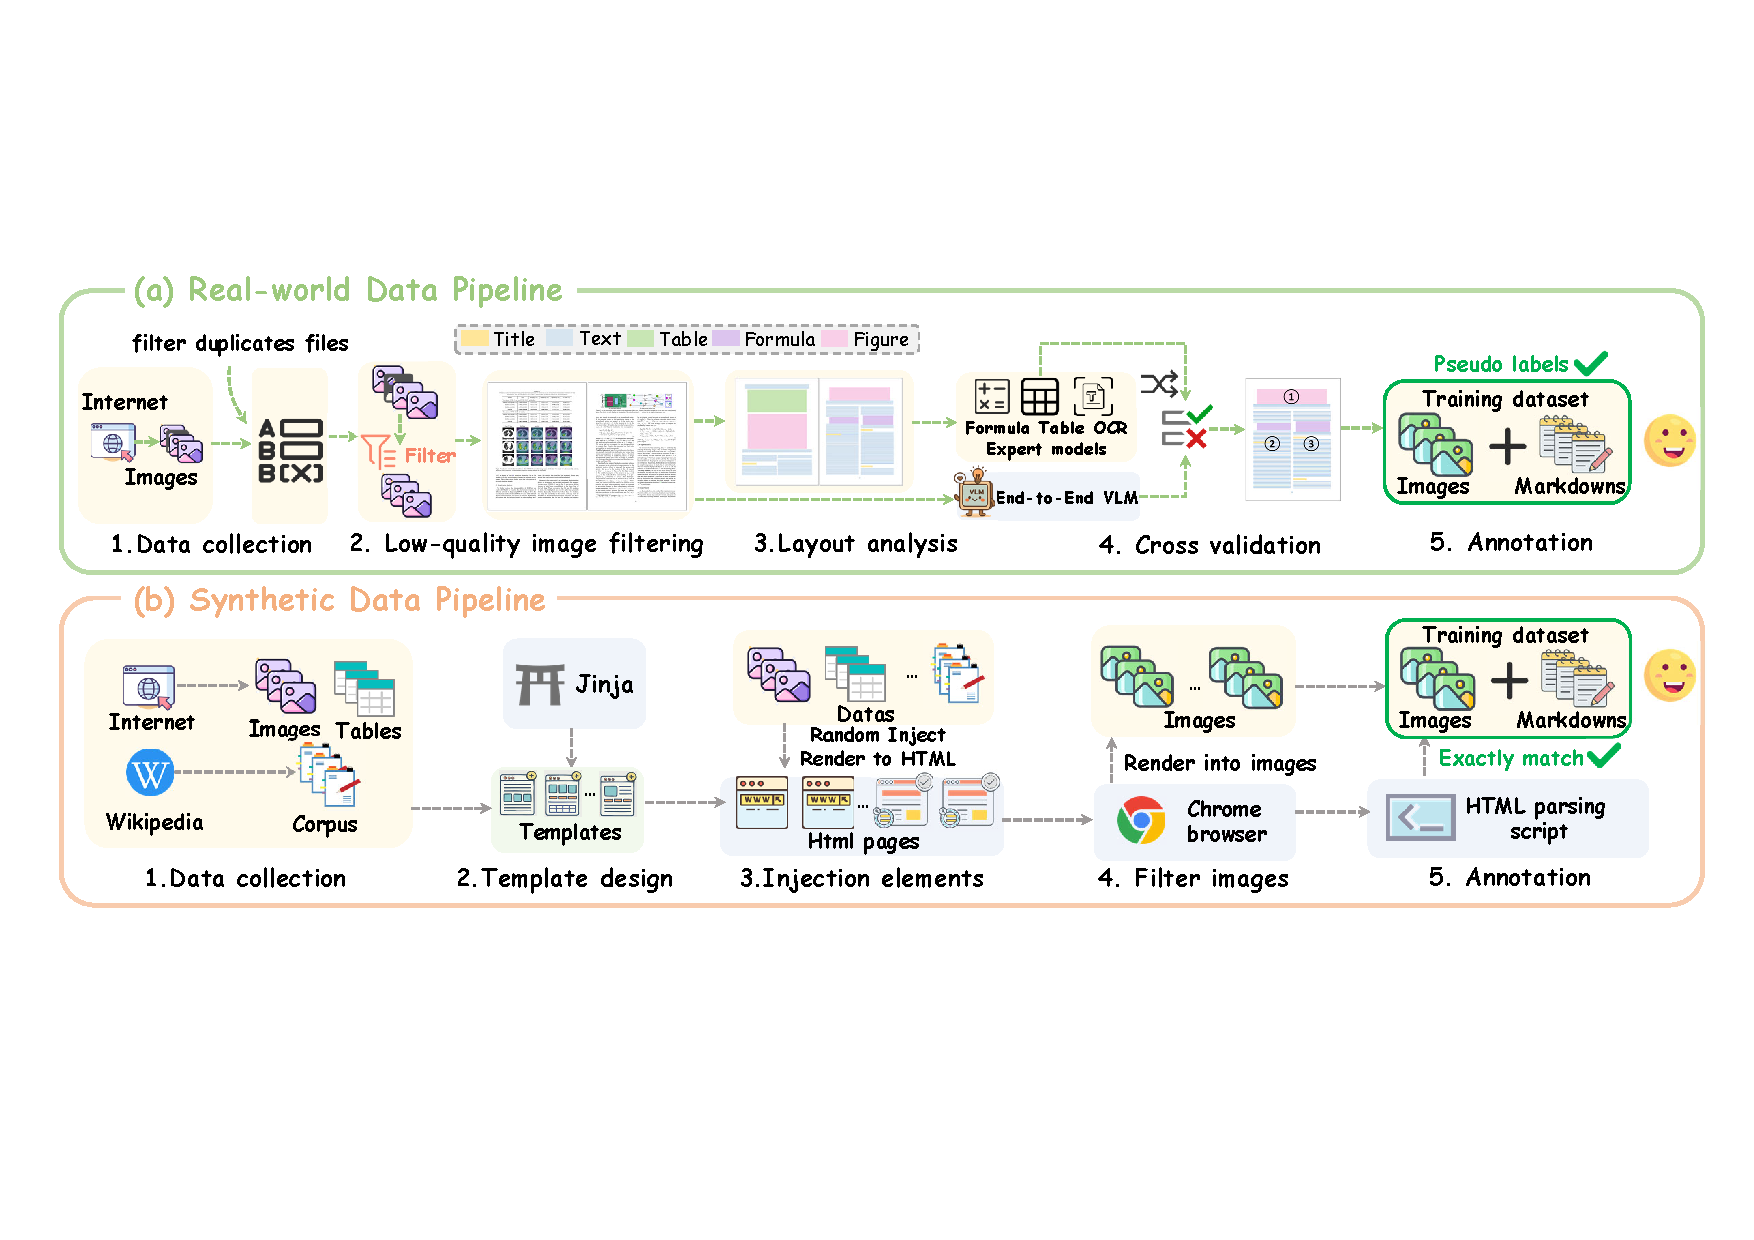
\includegraphics[width=1\linewidth]{picture/figure2_V2.pdf}
  \vspace{-2mm}
  \caption{ Data construction pipelines for document parsing.  (a) Real-world pipelines enhance quality by combining multiple expert models and layout analysis, yielding better-aligned supervision through intersection and reading order reasoning. (b) Synthetic pipeline leverages structured HTML templates and browser rendering to generate clean, exactly-aligned scanned document parsing data, ensuring high-quality supervision for end-to-end parsing. }
  \label{fig:example111}
% \vspace{-3mm}
\end{figure}





\subsection{RL with Layout-Aware Rewards}
As illustrated in Figure~\ref{fig:example222}, we employ an RL framework to directly optimize scanned document parsers, aiming to enhance both structural fidelity and semantic accuracy. Specifically, we utilize GRPO~\citep{shao2024deepseekmath}, which enables learning from rule-based reward signals without relying on absolute values. GRPO operates by generating a set of candidate Markdown outputs for each document and evaluating them using a \textit{multi-aspect reward}, denoted as $R_{\text{Multi-Aspect}}$, which integrates multiple rule-based criteria into a unified supervisory signal. These raw rewards are then converted into relative advantage scores by comparing each candidate against others within the same group. This relative evaluation promotes training stability and encourages the selection of higher-quality outputs, eliminating the need for a learned value function or critic. Notably, our reinforcement learning approach avoids any explicit thinking or intermediate reasoning process; instead, all outputs are treated as final answers, with the model receiving verifiable rewards based on these outputs.

The multi-aspect reward $R_{\text{Multi-Aspect}}$ consists of three complementary components, each capturing a different aspect of parsing quality: 






\paragraph{Edit Distance Reward ($R_{\mathrm{dist}}$)}  
We define the edit distance reward based on the normalized Levenshtein distance \( D(y, \hat{y}) \) between the predicted output \( \hat{y} \) and the reference output \( y \):

\vspace{-3mm}
\begin{equation}
R_{\text{dist}} = 1 - \tfrac{D(y, \hat{y})}{\max(N, M)}
\end{equation}
\vspace{-3mm}

where \( N = |y| \) and \( M = |\hat{y}| \) are the lengths of the reference and predicted sequences, respectively. The distance \( D(y, \hat{y}) \) measures the minimum number of single-character insertions, deletions, or substitutions required to convert \( \hat{y} \) into \( y \), thereby capturing both semantic and formatting discrepancies. This reward is bounded within \([0, 1]\), with higher values indicating better alignment between prediction and reference. Meanwhile, the reference output \( y \) is synthesized through two data generation pipelines proposed in this work. It is produced with rigorous rule-based filtering and consistency validation, and serves as a high-quality surrogate for ground-truth annotations in evaluating the quality of the model output.





\begin{figure}[t]
  \centering
  % 插入图片，options 中可以设置宽度、高度、缩放比例等
  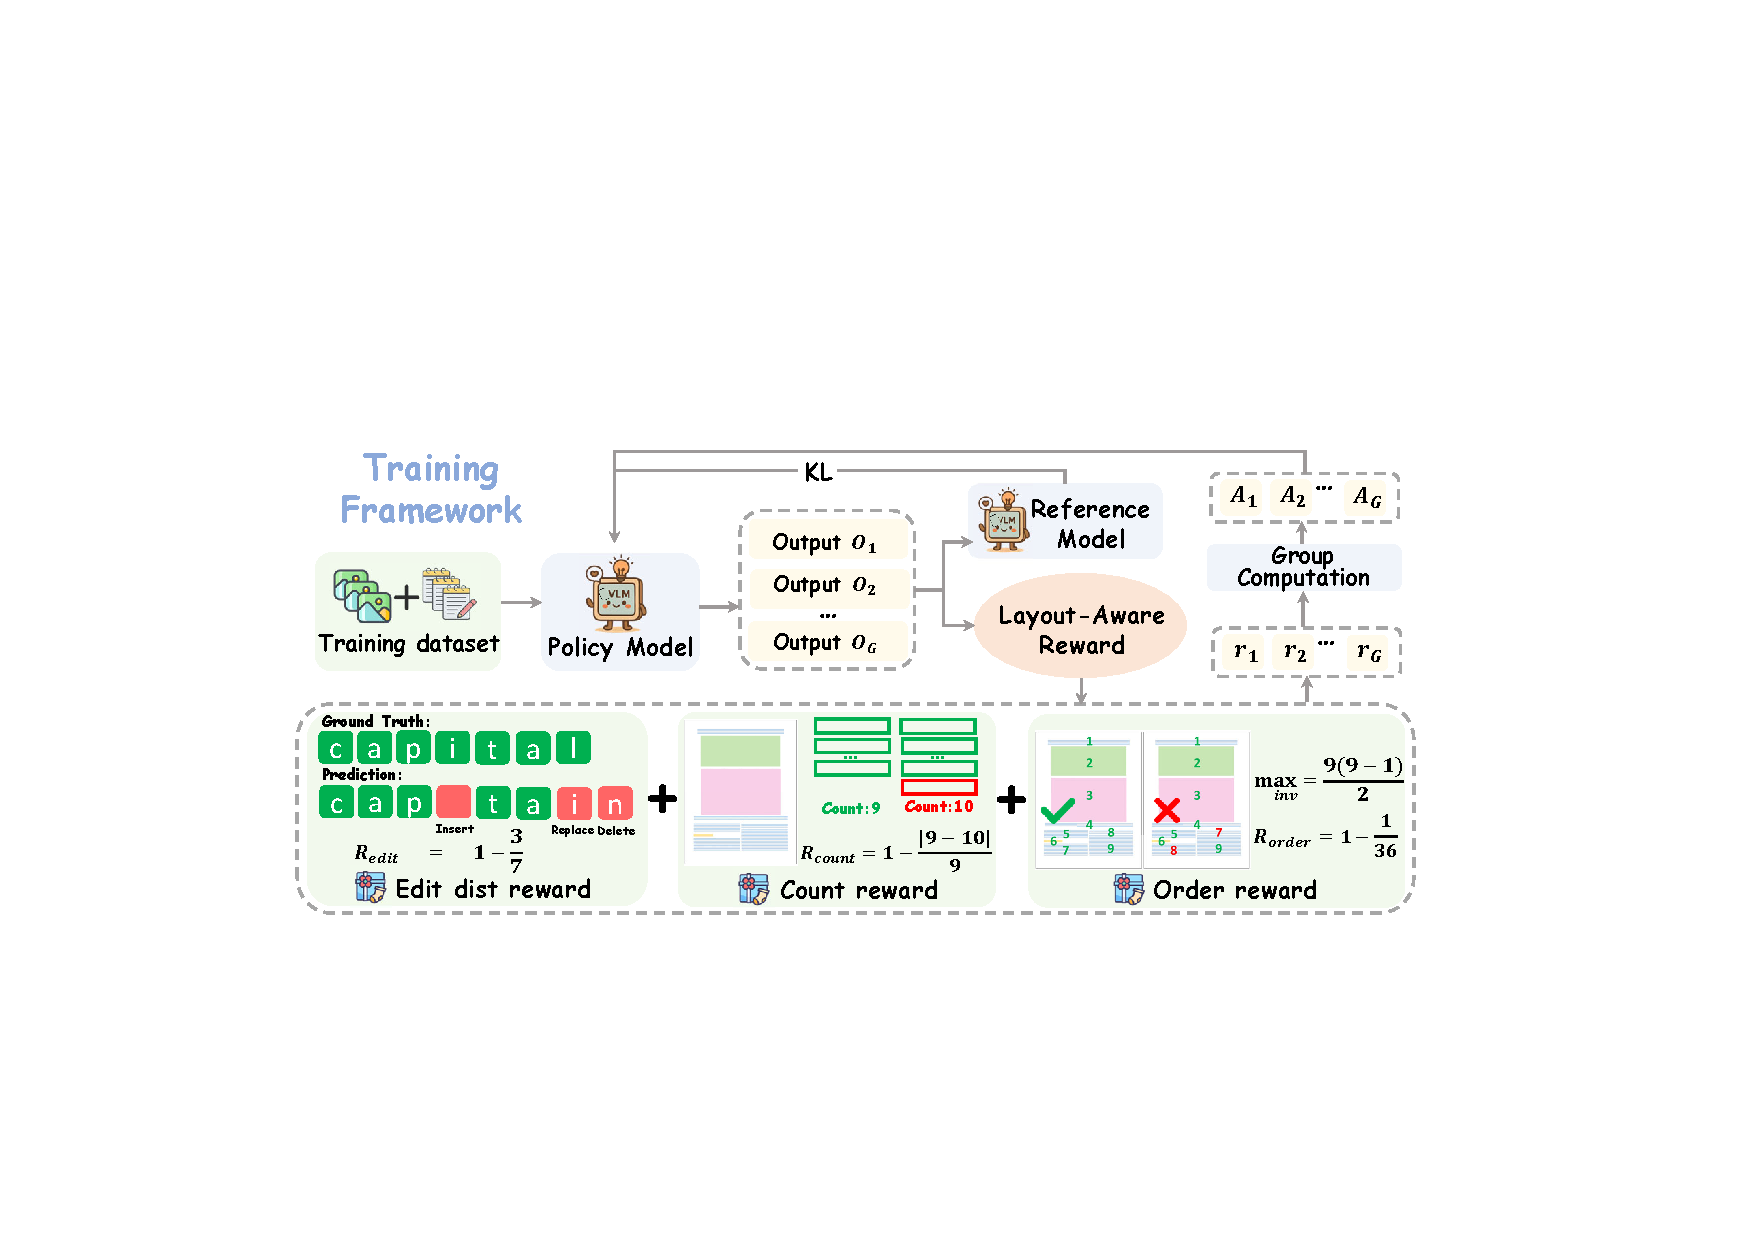
\includegraphics[width=0.98\linewidth]{picture/figure3_V10.pdf}
  % \vspace{-1mm}
  \caption{Overview of Infinity-Parser training framework. Our model is optimized via reinforcement finetuning with edit distance, layout, and order-based rewards. 
  }
  \label{fig:example222}
  % \vspace{-5mm}
\end{figure}



\paragraph{Count Reward ($R_{\mathrm{count}}$)}
To encourage accurate paragraph segmentation, let $N_Y$ and $N_{\hat Y}$ be the numbers of reference and predicted paragraphs. We define:

\vspace{-3mm}
\begin{equation}
R_{\text{count}} = 1 - \tfrac{|N_Y - N_{\hat{Y}}|}{N_Y}
\end{equation}
\vspace{-3mm}
 
which penalizes missing or spurious paragraphs.

\paragraph{Order Reward ($R_{\mathrm{order}}$)}
We measure sequence-level fidelity by counting pairwise inversions $D_{\mathrm{order}}$ between reference and predicted paragraphs. with $\max_{\mathrm{inv}}=N_Y(N_Y-1)/2$, we set:

\vspace{-3mm}
\begin{equation}
R_{\text{order}} = 1 - \frac{D_{\text{order}}}{\max_{\text{inv}}}
\end{equation}

rewarding preservation of the original reading order.


The final multi-aspect reward is a weighted combination of these three components. Specifically, we begin by applying the Hungarian algorithm~\citep{kuhn1955hungarian} to establish the optimal one-to-one matching between predicted and ground-truth segments, identifying both pairings and their relative order. Based on the matched segment count, we compute the count reward to reflect alignment in the number of segments. Using the relative sequence of matched pairs, we calculate the order reward to measure structural consistency. On top of these matchings, we compute the edit reward by averaging the edit similarities of each matched segment pair.  Combining these terms yields the final reward:

\vspace{-3mm}
\begin{equation}
R_{\text{Multi-Aspect}} = R_{\text{dist}} + R_{\text{count}} + R_{\text{order}}
\end{equation}


This multi-aspect design balances content fidelity with structural correctness and order preservation, providing rich supervision for end-to-end document parsing.


